\subsection{Aantal inputs}
Het aantal inputs heeft vooral invloed op de ratio van enen en nullen als antwoord. In dit experiment kijken we of het neurale netwerk verschillende hoeveelheden inputs correct kan beantwoorden en of het netwerk sneller leert van meer inputs.

\begin{table}[ht]
    \centering
      $\begin{array}{c||c|c |}
        \text{Aantal inputs} & \text{Aantal correct} & \text{Percentage \% correct} \\ \hline
        2 & 20 & 40 \\ \hline
        4 & 18 & 36 \\ \hline
        6 & 32 & 64 \\ \hline
        0 & 48 & 96 \\ \hline
        10 & 50 & 100 \\ \hline
        12 & 50 & 100 \\ \hline
        14 & 50 & 100 \\ \hline
      \end{array}$
    \caption{Aantal correcte antwoorden over 50 executies met verschillende aantallen inputs}
    \label{tab:inputs}
\end{table}

\begin{figure}[ht!]
    \centering
    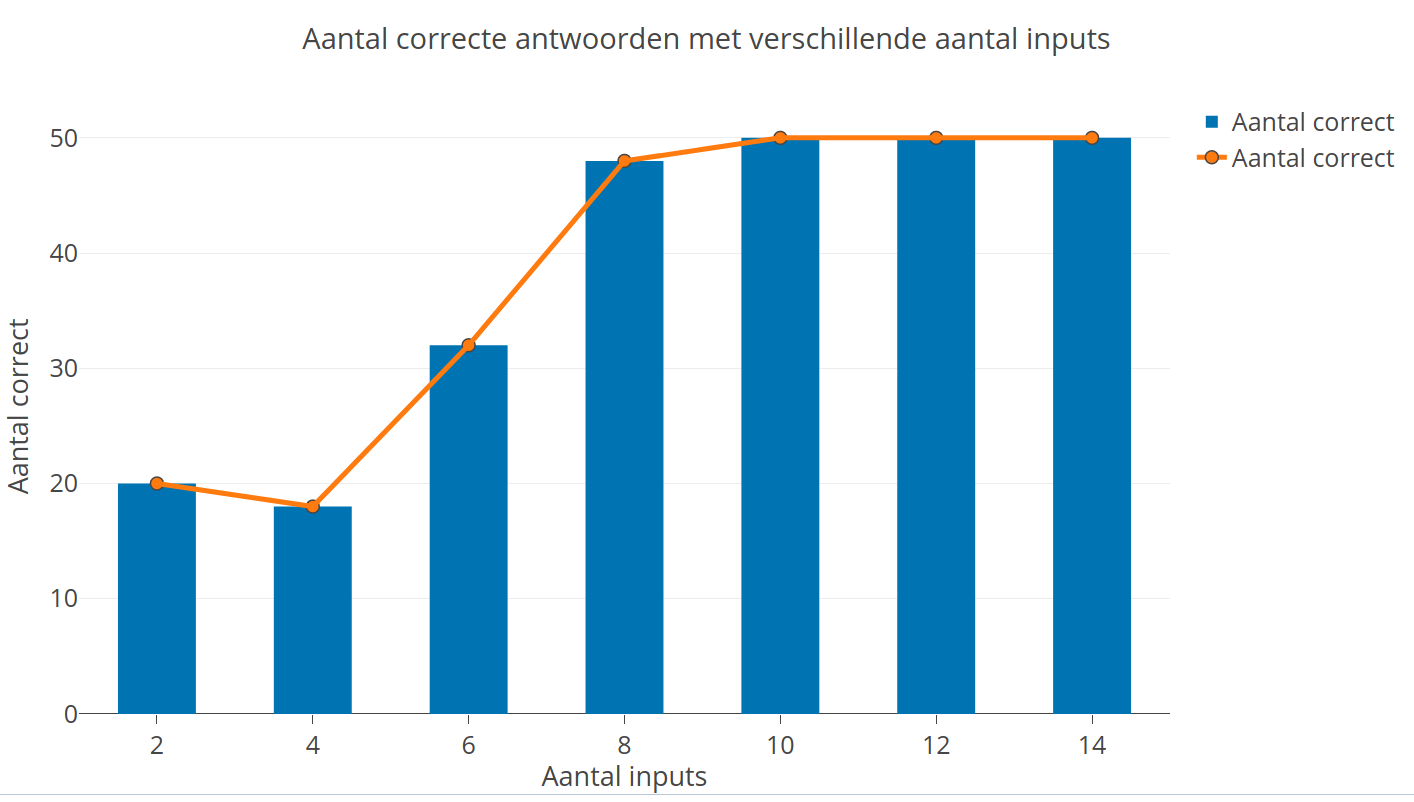
\includegraphics[scale=0.3]{graphs/inputs.png}
    \caption{Grafiek van Tabel \ref{tab:inputs}}
    \label{fig:inputs}
\end{figure}